\newpage
\subsection{\MsPacManName}

Two clusterings are examined for \MsPacManName (Table~\ref{tab:qualitative_ms_pacman_metrics}), obtained at layer 6b with $K=3$ and at layer 4 with $K=5$.

Both clusterings are organized around the same high-level concept, the progress of the episode, tracked through the score and the number of pellets remaining in the maze, rather than a spatial feature of the observation as in \MarioBrosName.
With $K=3$ (Figure~\ref{fig:qualitative_ms_pacman}), the partition separates the start (cluster A), the middle (cluster B), and the end (cluster C) of the episode.
With $K=5$ (Figure~\ref{fig:qualitative_ms_pacman_alt}), the same axis is cut more finely: the very start of the episode with a null score (cluster D), the early episode in which most pellets remain (cluster E), two clusters of the late episode in which few pellets remain (clusters F and G), which are hard to distinguish visually, and the end of the episode (cluster H).
The two clusterings are equally consistent across surrogate policies (\gls{cu} of $0.88$ in both cases), but the one at layer 4 is less abstract (\gls{as} of $0.47$ against $0.52$), which lowers its \gls{acu} ($0.35$ against $0.40$).

\vfill
\begin{table}[H]
    \centering
    \begin{tblr}{
        colspec={c c c c c},
        rowsep=2pt,
        hline{1,Z} = {1pt},
        hline{5} = {0.5pt},
        hline{2,6} = {0.3pt},
        row{1,5} = {bg=black!8, font=\bfseries},
        column{1} = {font=\bfseries}
    }
        Layer 6b & $K=3$ & \gls{cu} 0.88 $\pm$0.01 & \gls{as} 0.52 $\pm$0.01 & \gls{acu} 0.40 $\pm$0.01 \\
        A & \SetCell[c=4]{l} Start of the episode. & & & \\
        B & \SetCell[c=4]{l} Middle of the episode. & & & \\
        C & \SetCell[c=4]{l} End of the episode. & & & \\
        Layer 4 & $K=5$ & \gls{cu} 0.88 $\pm$0.01 & \gls{as} 0.47 $\pm$0.00 & \gls{acu} 0.35 $\pm$0.00 \\
        D & \SetCell[c=4]{l} Very start of the episode, null score. & & & \\
        E & \SetCell[c=4]{l} Early in the episode, most pellets remain. & & & \\
        F & \SetCell[c=4]{l} Late in the episode, few pellets remain. & & & \\
        G & \SetCell[c=4]{l} Late in the episode, few pellets remain (hard to distinguish from cluster F). & & & \\
        H & \SetCell[c=4]{l} End of the episode, almost no pellets remain. & & & \\
    \end{tblr}
    \caption{\gls{cu}, \gls{as}, and \gls{acu} of the two clusterings analyzed in the \MsPacManName environment, followed by the description of the clusters shown in Figures~\ref{fig:qualitative_ms_pacman} and~\ref{fig:qualitative_ms_pacman_alt}.}
    \label{tab:qualitative_ms_pacman_metrics}
\end{table}
\vfill

\newpage
\vspace*{\fill}
\begin{figure}[t]
    \centering
    \resizebox{\textwidth}{!}{
    \begin{tikzpicture}

    \node (ligne_1) at (0, 0) {};

    \node[] at ($(ligne_1) + (-4.5cm, 0cm)$) {
    \begin{minipage}{4.5cm}
        \centering
        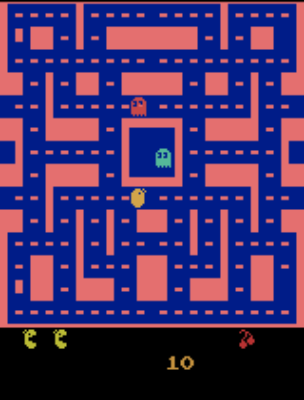
\includegraphics[width=2cm]{figures/clustering_agent_representation/pictures/ms_pacman/qualitative/cluster_1/image_1.png}
        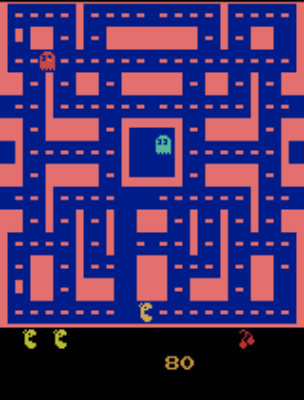
\includegraphics[width=2cm]{figures/clustering_agent_representation/pictures/ms_pacman/qualitative/cluster_1/image_2.png}

        \small Start of the episode.
    \end{minipage}
    };

    \node[] at ($(ligne_1) + (0cm, 0cm)$) {
    \begin{minipage}{4.5cm}
        \centering
        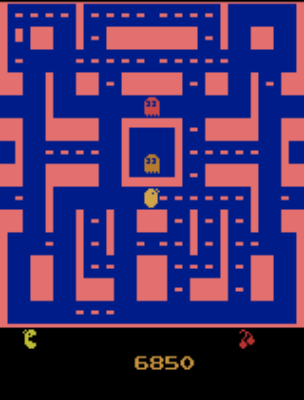
\includegraphics[width=2cm]{figures/clustering_agent_representation/pictures/ms_pacman/qualitative/cluster_0/image_1.png}
        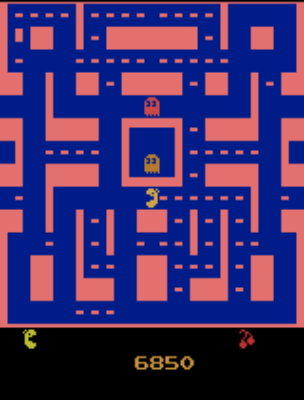
\includegraphics[width=2cm]{figures/clustering_agent_representation/pictures/ms_pacman/qualitative/cluster_0/image_2.png}

        \small Middle of the episode.
    \end{minipage}
    };

    \node[] at ($(ligne_1) + (4.5cm, 0cm)$) {
    \begin{minipage}{4.5cm}
        \centering
        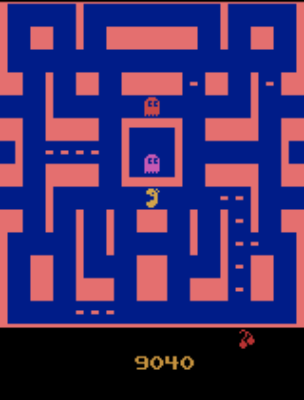
\includegraphics[width=2cm]{figures/clustering_agent_representation/pictures/ms_pacman/qualitative/cluster_2/image_1.png}
        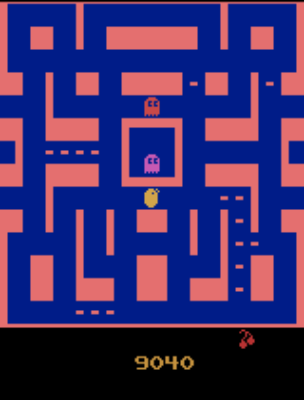
\includegraphics[width=2cm]{figures/clustering_agent_representation/pictures/ms_pacman/qualitative/cluster_2/image_2.png}

        \small End of the episode.
    \end{minipage}
    };

    \end{tikzpicture}
    }
    \caption{Clusters identified by \gls{car} in the Ms.\ Pac-Man environment (layer 6b, $K=3$).}
    \label{fig:qualitative_ms_pacman}
\end{figure}


\begin{figure}[H]
    \qualitativeClusterFigureSetup
    \qualitativeClusterTwo
        {figures/clustering_agent_representation/pictures/ms_pacman/qualitative_alt/cluster_0/image_1.png}
        {figures/clustering_agent_representation/pictures/ms_pacman/qualitative_alt/cluster_0/image_2.png}
        {D}
    \qualitativeClusterTwo
        {figures/clustering_agent_representation/pictures/ms_pacman/qualitative_alt/cluster_1/image_1.png}
        {figures/clustering_agent_representation/pictures/ms_pacman/qualitative_alt/cluster_1/image_2.png}
        {E}
    \qualitativeClusterTwo
        {figures/clustering_agent_representation/pictures/ms_pacman/qualitative_alt/cluster_2/image_1.png}
        {figures/clustering_agent_representation/pictures/ms_pacman/qualitative_alt/cluster_2/image_2.png}
        {F}
    \qualitativeClusterTwo
        {figures/clustering_agent_representation/pictures/ms_pacman/qualitative_alt/cluster_3/image_1.png}
        {figures/clustering_agent_representation/pictures/ms_pacman/qualitative_alt/cluster_3/image_2.png}
        {G}
    \qualitativeClusterTwo
        {figures/clustering_agent_representation/pictures/ms_pacman/qualitative_alt/cluster_4/image_1.png}
        {figures/clustering_agent_representation/pictures/ms_pacman/qualitative_alt/cluster_4/image_2.png}
        {H}
    \caption{Clusters D--H identified by \gls{car} in the \MsPacManName environment (layer 4, $K=5$).}
    \label{fig:qualitative_ms_pacman_alt}
\end{figure}

\vfill
